\documentclass{beamer}
\usetheme{Boadilla}

\usepackage{hyperref}
% \usepackage{biblatex}
% \addbibresource{references.bib}

\usepackage{graphicx}
\graphicspath{ {results} }

\title[ML for Cancer Diagnosis] {
    Machine Learning for Cancer Diagnosis on Microarray Data
}
\author[Pacchione, Rollo, Vandenberg, Wadas] {
    Ty Pacchione, Danny Rollo, Alexander Vandenberg, \\ and Mitchell Wadas
}
\date {
    December 7, 2023
}

\setbeamersize{text margin left=7mm,text margin right=10mm} 
\renewcommand{\raggedright}{\leftskip=0pt \rightskip=0pt}

\begin{document}

    \frame{\titlepage}

    \iffalse
    \begin{frame}
        \frametitle{Outline}
        \tableofcontents
    \end{frame}
    \fi

    \begin{frame}{Background}
        \begin{itemize}\setlength\itemsep{15pt}
            \item {
                Microarrays measure the expression of thousands of genes simultaneously. 
            }
            \item {
                Microarray data is increasingly being used for early diagnosis of cancer.
            }
            \item {
                Researchers are struggling to extract meaningful information from so much data.
            }
            \item {
                We propose an application of machine learning to make diagnoses from microarray data.
            }
        \end{itemize}
    \end{frame}
    
    \begin{frame}{Data}
        \begin{itemize} \setlength\itemsep{15pt}
            \item {
                Raw data was sourced from the Structural Bioinformatics and Computational Biology Lab's
                CuMiDa database \cite{CuMiDa}. 
                Each file corresponds to a specific type of cancer and set of genes. 

                \begin{center}
                    \vspace{10pt}
                    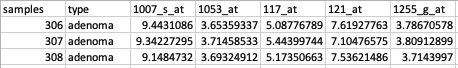
\includegraphics[scale=.6]{SampleScreenshot.png}
                \end{center}
            }
            \item {
                We downloaded approximately 40 datasets corresponding to different cancer / gene set
                combinations.
            }
            \item {
                We combined them into two datasets, one corresponding to each gene set.
            }
        \end{itemize}
    \end{frame}

    \begin{frame}{Procedure}
        \begin{itemize} \setlength\itemsep{15pt}
            \item {
                We formulated the diagnosis as a multi-class classification problem.
            }
            \item {
                A notable characteristic of our data is the number of features, between
                30,000 and 50,000.
            }
            \item {
                We compared traditional ML (logistic regression with PCA) 
                and deep learning.
            }
            \item {
                We compared different set of genes (as features) to determine which
                has more diagnostic power.
            }
        \end{itemize}
    \end{frame}

    \begin{frame}{Methods - Logistic Regression with PCA}
        \begin{itemize} \setlength\itemsep{15pt}
            \item {
                We decomposed the data into 50 principal components which captured
                roughly 95\% of the variance (efficient reduction).
            }
            \item {
                We applied logistic regression to the principal components.
            }
        \end{itemize}
    \end{frame}

    \begin{frame}{Methods - Neural Network}
        \begin{itemize} \setlength\itemsep{15pt}
            \item {
                Instead of using PCA, we gave the network the full feature set, allowing it to
                perform feature extraction.
            }
            \item {
                We performed grid search hyperparameter optimization to find the optimal neural
                architecture.
            }
        \end{itemize}
    \end{frame}

    \begin{frame}{Cross Validation Results}
        \begin{center}
            \hspace{10pt}
            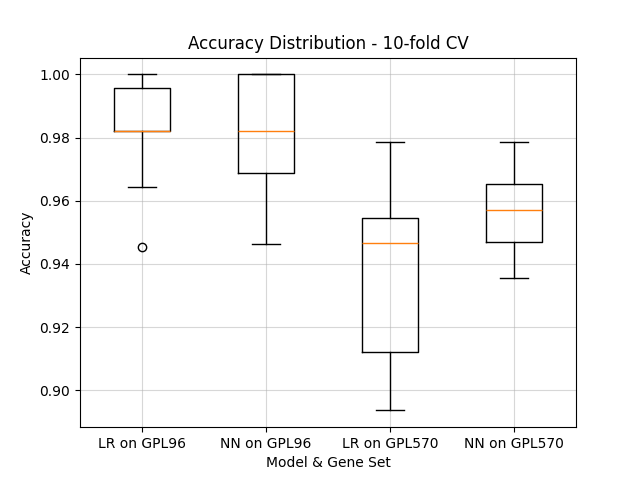
\includegraphics[scale=.65]{AccuracyDist.png}
        \end{center}
    \end{frame}

    \begin{frame}{Confusion Matrix - GPL96}
        \begin{center}
            \hspace{-60pt}
            \begin{minipage}{0.4\textwidth}
                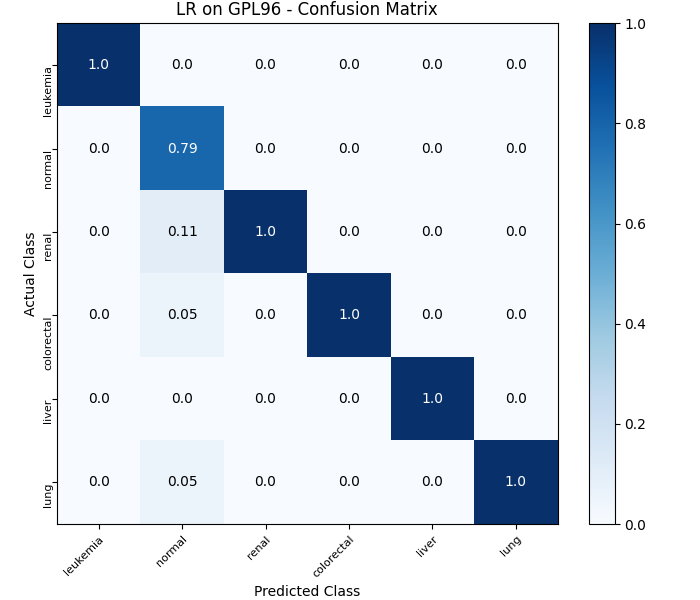
\includegraphics[scale=.40]{LRonGPL96Confusion.png}
            \end{minipage}
            \hspace{30pt}
            \begin{minipage}{0.4\textwidth}
                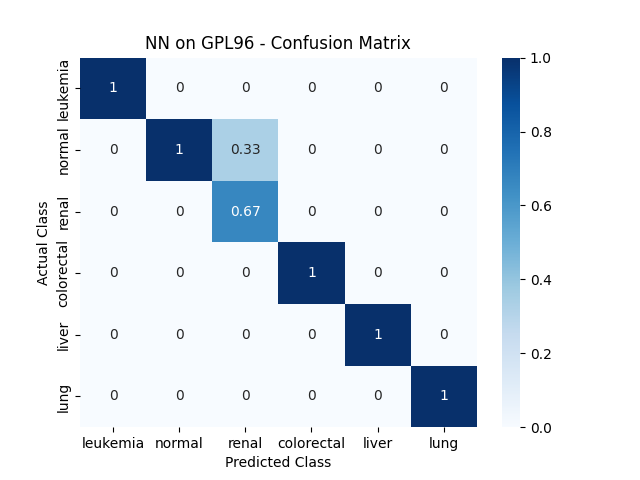
\includegraphics[scale=.40]{NNonGPL96Confusion.png}
            \end{minipage}
        \end{center}
    \end{frame}

    \begin{frame}{Confusion Matrix - GPL570}
        \begin{center}
            \hspace{-60pt}
            \begin{minipage}{0.4\textwidth}
                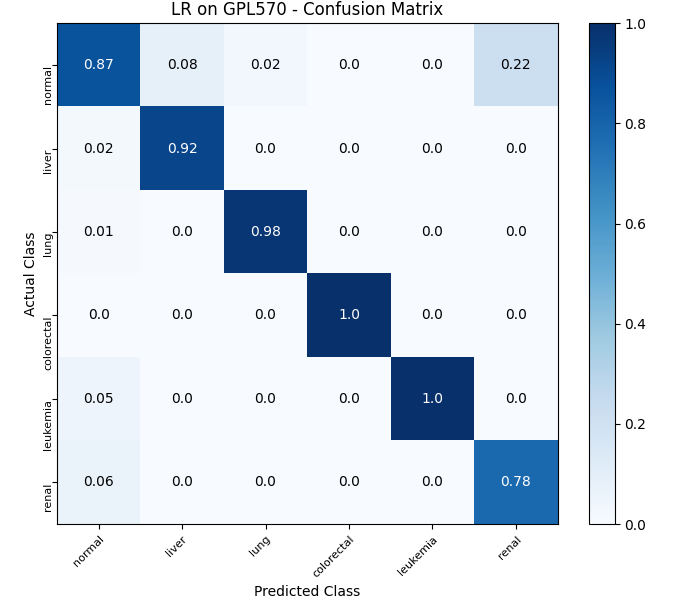
\includegraphics[scale=.40]{LRonGPL570Confusion.png}
            \end{minipage}
            \hspace{30pt}
            \begin{minipage}{0.4\textwidth}
                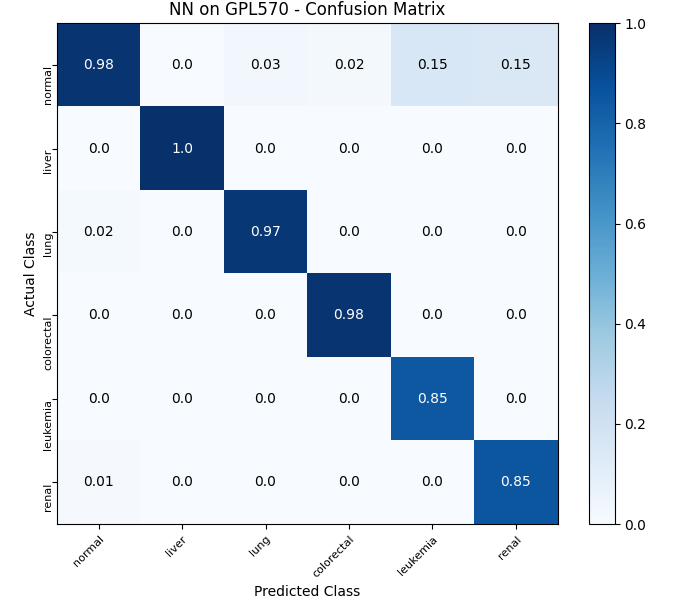
\includegraphics[scale=.40]{NNonGPL570Confusion.png}
            \end{minipage}
        \end{center}
    \end{frame}

    \begin{frame}{Feature Analysis - GPL96}
        \begin{center}
            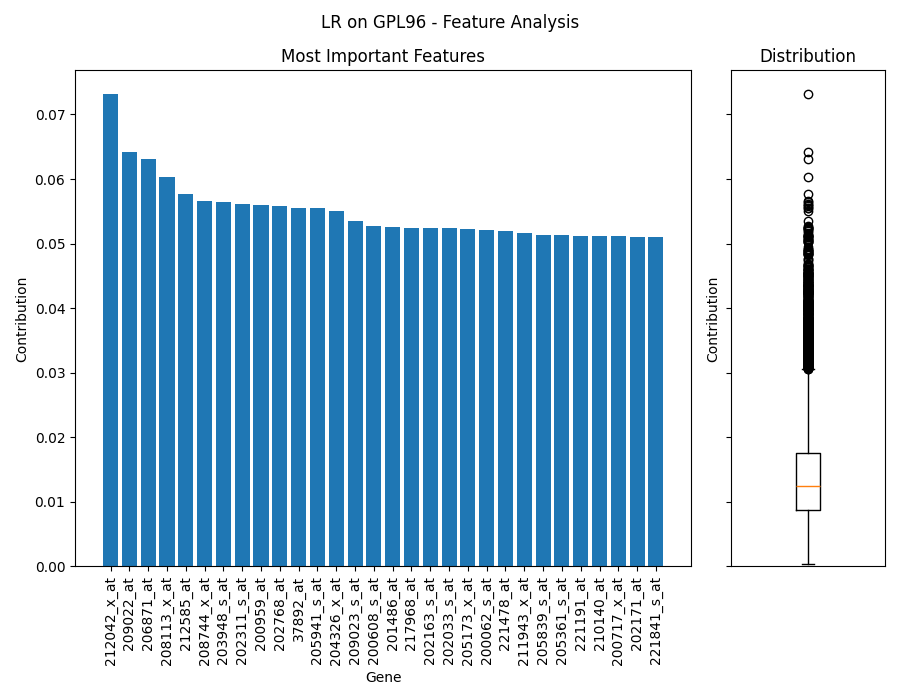
\includegraphics[scale=.45]{LRonGPL96Features.png}
        \end{center}
    \end{frame}

    \begin{frame}{Feature Analysis - GPL570}
        \begin{center}
            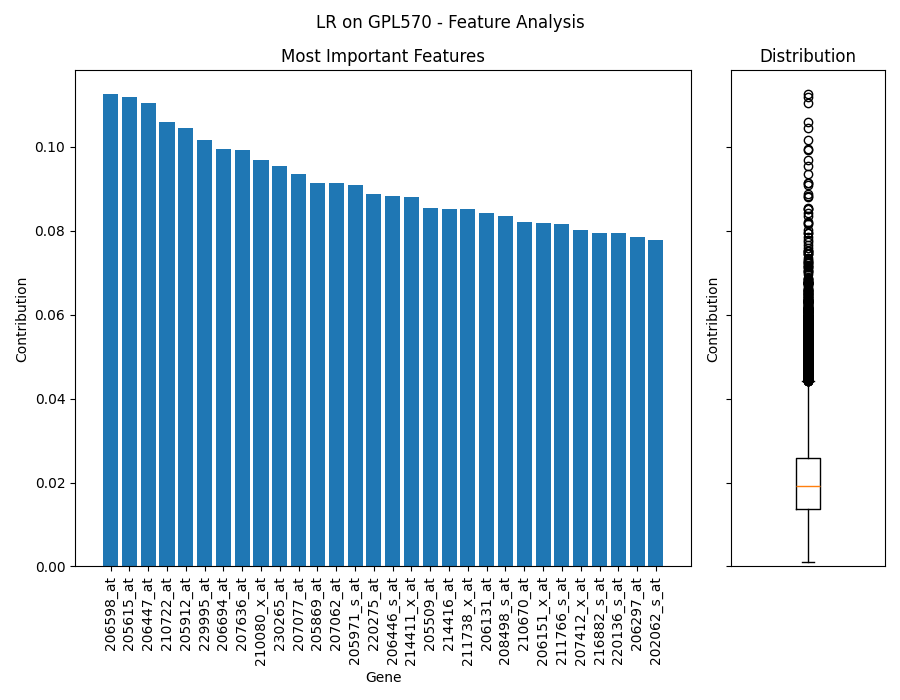
\includegraphics[scale=.45]{LRonGPL570Features.png}
        \end{center}
    \end{frame}

    \iffalse % not sure these add value, also very hard to see.
    \begin{frame}{ROC Curve - GPL96}
        \begin{center}
            \hspace{-60pt}
            \begin{minipage}{0.4\textwidth}
                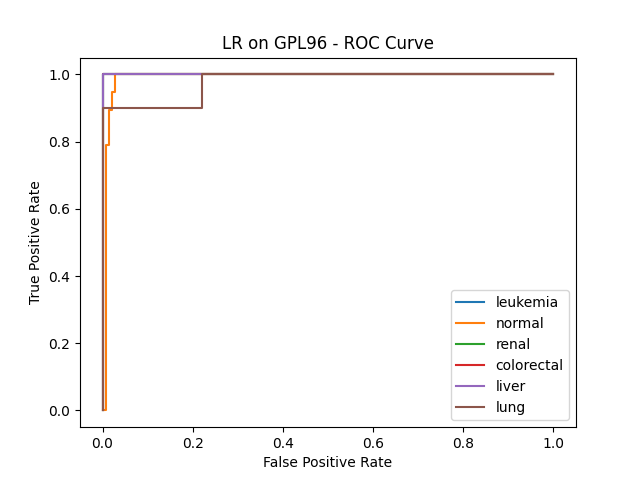
\includegraphics[scale=.4]{LRonGPL96ROC.png}
            \end{minipage}
            \hspace{40pt}
            \begin{minipage}{0.4\textwidth}
                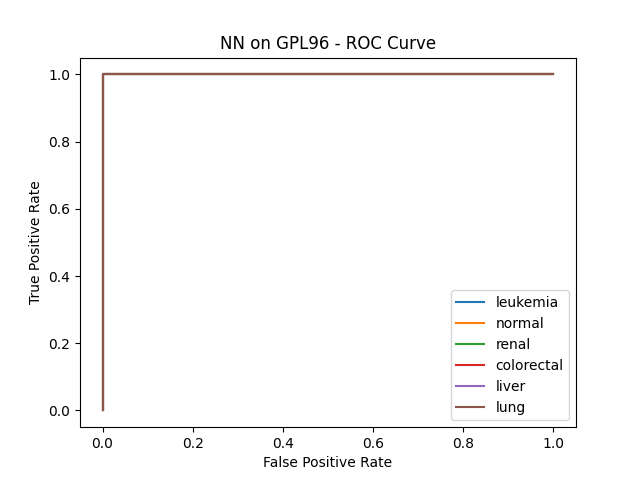
\includegraphics[scale=.4]{NNonGPL96ROC.png}
            \end{minipage}
        \end{center}
    \end{frame}

    \begin{frame}{ROC Curve - GPL570}
        \begin{center}
            \hspace{-60pt}
            \begin{minipage}{0.4\textwidth}
                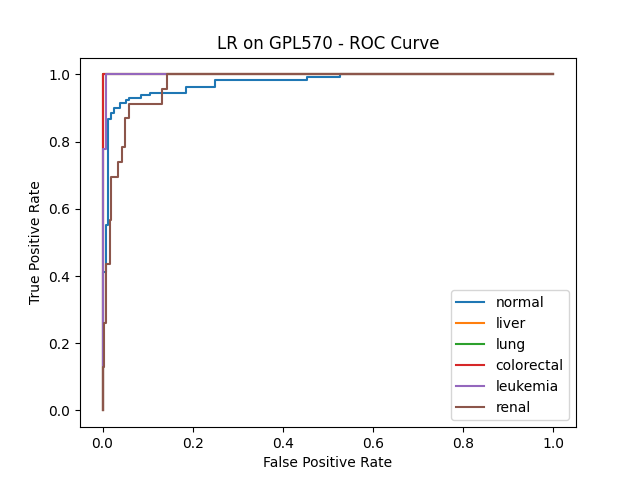
\includegraphics[scale=.4]{LRonGPL570ROC.png}
            \end{minipage}
            \hspace{40pt}
            \begin{minipage}{0.4\textwidth}
                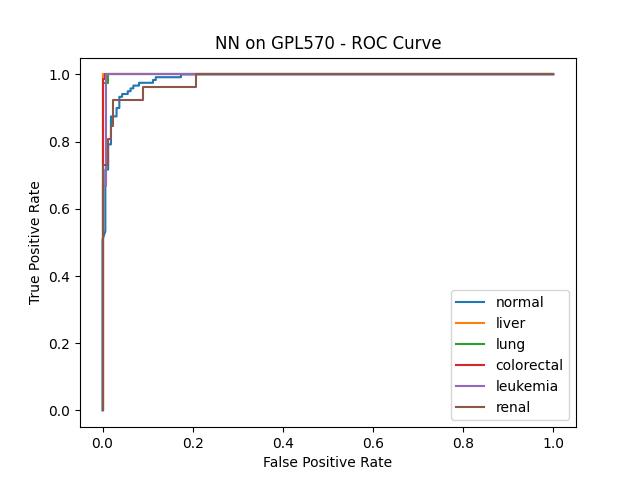
\includegraphics[scale=.4]{NNonGPL570ROC.png}
            \end{minipage}
        \end{center}
    \end{frame}
    \fi
    
    \begin{frame}{References}
        % \nocite{*}
        % \printbibliography
    \end{frame}

\end{document}